\documentclass[12pt, french]{article}

\usepackage{fancyhdr, fancybox, lastpage, makecell,amssymb}
\usepackage[most]{tcolorbox}
\usepackage[a4paper, margin={0.3in, .75in}]{geometry}
\usepackage{wrapfig}
\pagestyle{fancy}
\renewcommand\headrulewidth{1pt}
\renewcommand\footrulewidth{1pt}
\fancyhf{}
\rhead{ \em{Zakaria Haouzan}}
\lhead[C]{\em{2ème année baccalauréat SM-X}}
\chead[C]{}
\rfoot[C]{\emph{Les Ondes Mécaniques Périodiques}}
\lfoot[R]{ \emph{Exercices Supplémentaires}}
\cfoot[]{\em{Page \thepage / \pageref{LastPage}}}


\newtcolorbox{Box2}[2][]{
                lower separated=false,
                colback=white,
colframe=white!20!black,fonttitle=\bfseries,
colbacktitle=white!30!gray,
coltitle=black,
enhanced,
attach boxed title to top left={yshift=-0.1in,xshift=0.15in},
title=#2,#1}


\begin{document}
\begin{center}
   \shadowbox {\bf{Les Ondes Mécaniques Progressives
Périodiques}}
\end{center}

\vspace{-0.2cm}
%%_________________________Exercice ! :"_________________________Exercice
%   \begin{center}
	   %\vspace{-0.6cm}
	%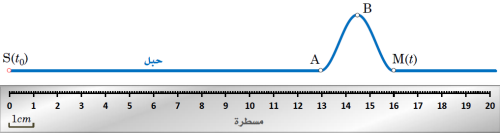
\includegraphics[width=0.6\textwidth ]{./img/Exercice01.png}
  %\end{center}



\begin{Box2}{\textbf{Exercice 1 :Propagation d'une onde le long d'une corde }}
Une lame vibrante en mouvement sinusoïdal de fréquence N, fixée à l'extrémité S d'une corde élastique SA très longue et tendue horizontalement, génère le long de celle-ci une onde progressive périodique non amortie de célérité v.  Un dispositif approprié, placé en A, empêche toute réflexion des ondes.

Le mouvement de S débute à l'instant t = 0.

Les courbes (1) et (2) de la figure ci-dessous représentent l’élongation d'un point M de la corde, situé.
à la distance d de S, et l'aspect de la corde à un instant $t_1$ .

   \begin{center}
	   \vspace{-0.3cm}
	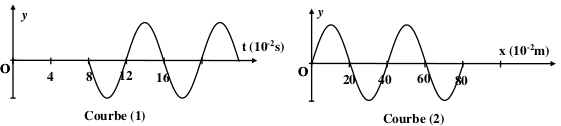
\includegraphics[width=0.6\textwidth ]{./img/Ex1.png}
  \end{center}

  \textbf{1- }Identifier, en justifiant, la courbe représentant l'aspect de la corde à l'instant $t_1$.

  \textbf{2- }Donner le nombre d'affirmations justes parmi les affirmations suivantes :
  
  \textbf{2.a- }Le phénomène de diffraction ne se produit jamais pour une onde mécanique.
  
  \textbf{2.b- }Les ondes progressives périodiques sinusoïdales se caractérisent par une périodicité temporelle et une périodicité spatiale.
  
  \textbf{2.c- }L'onde qui se propage le long de la corde est une onde longitudinale.

  \textbf{2.d- }La vitesse de propagation d'une onde mécanique ne dépend pas de l'amplitude de l'onde.

\textbf{3- }Par exploitation des courbes précédentes, déterminer :

\textbf{3.1- }La longueur d'onde $\lambda$, la période T et la célérité v de l'onde

\textbf{3.2- }Le retard temporel $\tau$ du point M par rapport à la source S de l'onde et déduire la distance d.

\textbf{4- }On donne la relation qui lie la célérité v de l'onde, la tension F de la corde et sa masse linéique $\mu$ (quotient de la masse sur la longueur) : $v = \sqrt{\frac{F}{\mu}}$

\textbf{4-1 }En utilisant les équations aux dimensions, vérifier l'homogénéité de la relation précédente.

\textbf{4.2- }La corde est-elle un milieu dispersif ? Justifier.


\textbf{4.3- }On double la tension F de la corde (F'= 2F ) sans modifier la fréquence N.
Déterminer dans ce cas la longueur d'onde $\lambda$.
\end{Box2}
%%_________________________Exercice !2 :"_________________________Exercice
\begin{tcolorbox}\textbf{Exercice 2 :L’échographie }
	\emph{L’échographie est un outil du diagnostic médical. Sa technique utilise une sonde à ultrasons.}

\end{tcolorbox}
\begin{wrapfigure}[6]{r}{0.36\textwidth}
  \begin{center}
	  \vspace{-0.6cm}
	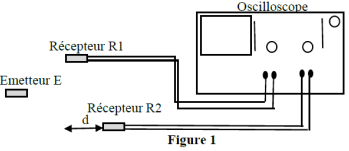
\includegraphics[width=0.36\textwidth]{./img/ex2_1.png}
  \end{center}
\end{wrapfigure}

	\textbf{ 1- Détermination de la célérité d’une onde
ultrasonore dans l’air}
	
On se propose de déterminer la célérité d’une onde
ultrasonore dans l’air à partir de la mesure de la
longueur d’onde $\lambda$ d’un signal émis par la sonde
d’un échographe de fréquence $N=40kHz$. Pour
cela on utilise un émetteur E produisant une
onde périodique sinusoïdale de même
fréquence que celle de sonde.

Les récepteurs $R_1$ et $R_2$ sont à égales distances de l'émetteur E. Lorsqu'on éloigne le récepteur $R_2$
d'une distance d (Figure 1), les deux sinusoïdes visualisées sur l'oscilloscope se décalent. Les deux
courbes sont en phase à chaque fois que la distance d entre $R_1$ et $R_2$ est un multiple entier n de $\lambda$
avec $n \in \mathbb{N}^*$.

\textbf{1.1- }Définir la longueur d'onde.

\textbf{1.2- } Choisir la réponse juste parmi les propositions suivantes :

\textbf{1.2.a- } Les ultrasons sont des ondes transportant la matière.

\textbf{1.2.b- }Les ultrasons sont des ondes mécaniques.

\textbf{1.2.c- }Les ultrasons se propagent avec la même vitesse dans tous les milieux.

\textbf{1.2.d- }Le domaine de la longueur d'onde des ondes ultrasonores est : $400 nm  \leq \lambda \leq 800 nm$.

\textbf{1.3- }Dans l'expérience réalisée, on relève pour n=12, la distance d= 10,2 cm. Déterminer la célérité de l’onde dans l'air.

\begin{wrapfigure}[8]{r}{0.26\textwidth}
  \begin{center}
	  \vspace{-1cm}
	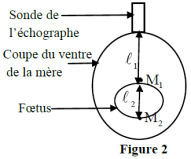
\includegraphics[width=0.26\textwidth]{./img/ex2_2.png}
  \end{center}
\end{wrapfigure}


\textbf{2- Application à l'échographie :\dotfill}

La sonde échographique utilisée est à la fois un émetteur et un
récepteur. Lorsque les ondes se propagent dans le corps humain, elles
sont en partie réfléchies par les parois séparant deux milieux différents.

La partie réfléchie de l'onde est reçue par la sonde puis analysée par
un système informatique.

La figure 2 représente le schéma du dispositif permettant
l'échographie d'un fœtus. Lors de l'examen, une salve d'ondes est émise
par l'émetteur de la sonde à la date t = 0. L'onde est réfléchie au point
$M_1$ et au point $M_2$ .

La sonde reçoit la première onde réfléchie à la date $t = t_1 = 80\mu{s}$ et la deuxième à la date $t =t_2 = 130\mu{s}$.

Trouver l'épaisseur $l_2$ du fœtus.

\begin{wrapfigure}[8]{r}{0.32\textwidth}
  \begin{center}
	  \vspace{-1.5cm}
	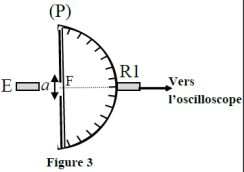
\includegraphics[width=0.32\textwidth]{./img/ex2_3.png}
  \end{center}
\end{wrapfigure}



\textbf{3- Diffraction de l'onde ultrasonore dans l’air :\dotfill}

Le schéma expérimental représenté sur la figure 3 comporte :

- L'émetteur E émettant l'onde ultrasonore de fréquence $N =40kHz$,

- Le récepteur R1 lié à un oscilloscope,

- Une plaque métallique (P) percée d'une fente (P) rectangulaire de largeur a très petite devant sa longueur,

-une feuille graduée permettant de mesurer les On déplace le récepteur $R_1$ dans le plan horizontal
d'un angle $\theta$ sur l'arc de cercle de centre F et de rayon $r = 40 cm$ et on note pour chaque
amplitude $U_m$ de l'onde reçue par $R_1$, l'angle $theta$ correspondant.

\textbf{3.1- }Comparer la longueur d'onde de l'onde tant. incidente avec celle de l'onde

\textbf{3.2- }On donne $a = 2,6 cm$. Trouver la distance du déplacement du récepteur pour observer le premier minimum d'amplitude $U_m$ de la tension du récepteur.


\begin{tcolorbox}\textbf{Exercice 3 :Les ondes ultrasonores }
\end{tcolorbox}
\emph{Les ondes ultrasonores sont des ondes de fréquence supérieure à celle des ondes sonores audibles par
l’homme. Elles sont exploitées dans plusieurs domaines, comme l’échographie.
Le but de cet exercice est :}

- L’étude de la propagation des ondes ultrasonores ;

- Détermination des dimensions d’un tube métallique.

\textbf{1- Propagation des ondes mécaniques :\dotfill}

\textbf{1.1.a- }Ecrire la définition de l’onde mécanique progressive.

\textbf{1.1.b- }Quelle est la différence entre l’onde mécanique longitudinale et l’onde mécanique transversale?

\textbf{1.2- }Propagation des ondes ultrasonores dans l’eau :
On pose un émetteur E et deux récepteurs $R_1$ et $R_2$ d’ondes ultrasonores dans une cuve remplie d’eau, de façon que l’émetteur et les deux récepteurs sont alignés suivant une règle graduée (Figure 1).

\begin{center}
	  \vspace{-0.5cm}
	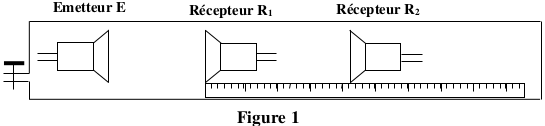
\includegraphics[width=0.8\textwidth]{./img/ex3_1.png}
  \end{center}

  \begin{wrapfigure}[10]{r}{0.33\textwidth}
  \begin{center}
	  \vspace{-0.6cm}
	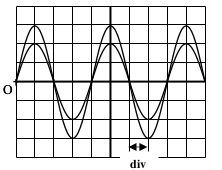
\includegraphics[width=0.33\textwidth]{./img/ex3_2.png}
  \end{center}
\end{wrapfigure}



L’émetteur émet une onde ultrasonore qui se propage dans l’eau
et arrive aux récepteurs $R_1$ et $R_2$. Les deux signaux captés par les
deux récepteurs $R_1$ et $R_2$, sont appliques successivement aux
entrées d’un oscilloscope.

Lorsque les deux récepteurs $R_1$ et $R_2$ se trouvent au zéro de la
règle, on constate sur l’écran de l’oscilloscope l’oscillogramme
représenté sur la figure 2, où les deux courbes correspondant aux
signaux captés par $R_1$ et $R_2$ sont en phases.

La sensibilité horizontale est fixée sur $5 \mu{s}/div$.

On éloigne $R_2$ suivant la règle graduée, on constate que la courbe correspondante au signal capté par
$R_2$ est décalée vers la droite. Les deux signaux captés par $R_1$ et $R_2$ deviennent à nouveau en phase, lorsque la distance entre $R_1$ et $R_2$ est $d = 3 cm$.

\textbf{1.2.a- }Ecrire la définition de la longueur d’onde $\lambda$.

\textbf{1.2.b- }Ecrire la relation entre la longueur d’onde $\lambda$, la fréquence N des ultrasons et sa célérité de
propagation dans un milieu quelconque.

\textbf{1.2.c- }En déduire de cette expérience, la valeur Ve de la célérité de propagation des ultrasons dans l’eau.

\textbf{1.3- Propagation des ultrasons dans l’air :\dotfill }

On conserve le même dispositif précédent $(d = 3 cm)$, et on vide la cuve, le milieu de propagation des ultrasons devient ainsi l’air. On observe que les deux courbes correspondant aux signaux captés par $R_1$ et $R_2$ ne sont plus en phases.

\textbf{1.3.a- }Expliquer le phénomène observé.

\textbf{1.3.b- }Calculer la valeur minimale de la distance de laquelle il faut éloigner le récepteur $R_2$ pour que les deux signaux deviennent à nouveau en phase.

On donne : La célérité de propagation des ultrasons dans l’air $V_a = 340 m/s$.


\begin{wrapfigure}{r}{0.32\textwidth}
  \begin{center}
	  \vspace{-0.6cm}
	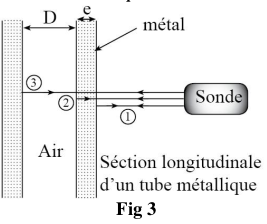
\includegraphics[width=0.32\textwidth]{./img/ex3_3.png}
	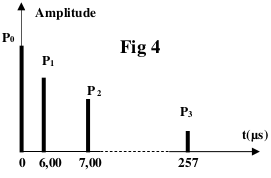
\includegraphics[width=0.32\textwidth]{./img/ex3_4.png}
  \end{center}
\end{wrapfigure}


\textbf{2- Utilisation des ultrasons pour mesurer les dimensions d’un tube métallique.}

Une sonde jouant le rôle d’un émetteur et récepteur, émet une
onde ultrasonore de courte durée dans une direction normale
à l’axe du tube cylindrique (Figure 3).

Cette onde traverse le tube et se réfléchit à chaque
changement de milieu de propagation, pour revenir à la
sonde, qui la transforme en signal électrique de courte durée.
On visualise à l’aide d’un oscilloscope à mémoire, les
signaux émis et reçus. L’oscillogramme obtenu au cours du
test fait sur le tube, a permis de tracer le diagramme de la
figure 4.

On observe des raies sous forme de pics verticaux : $P_0, P_1, P_2, P_3$. Figure 4.

- $P_0$ : correspond à l’instant de l’émission.

- $P_1$ : correspond à l’instant de la réception, par la sonde, de l’onde réfléchie 1.

- $P_2$ : correspond à l’instant de la réception, par la sonde, de l’onde réfléchie 2.

- $P_3$ : correspond à l’instant de la réception, par la sonde, de l’onde réfléchie 3. 

\underline{On donne : la vitesse de propagation des ultrasons .}

- Dans le métal du tube : $V_m = 1,00.10^4 m/s$.

- Dans l’air : $V_a$ = 340 m/s.

\textbf{2.1- }Trouver l’épaisseur e du métal du tube .

\textbf{2.2- }Trouver la valeur D du diamètre interne du tube.

\begin{Box2}{Exercice 4 :Les ondes ultrasonores }
\emph{On trouve parmi les applications des ondes ultrasonores, l’exploration du relief des fonds marins et la
localisation des regroupements de poissons, ce qui nécessite la connaissance de la vitesse de
propagation de ces ondes dans l’eau de mer.
Le but de cet exercice est de déterminer la vitesse de propagation d’une onde ultrasonore dans l’air et
dans l’eau de mer.}

\begin{wrapfigure}{r}{0.42\textwidth}
  \begin{center}
	  \vspace{-0.6cm}
	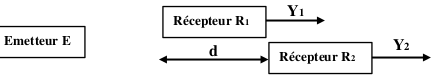
\includegraphics[width=0.42\textwidth]{./img/ex4_1.png}
  \end{center}
\end{wrapfigure}


\textbf{1- Détermination de la vitesse de propagation d’une onde ultrasonore dans l’air\dotfill}

On place un émetteur E d’ondes ultrasonores et deux récepteurs R1 et R2 comme l’indique la figure 1.

L’émetteur E envoie une onde ultrasonore progressive sinusoïdale qui se propage dans l’air. Celle-ci est captée par les deux récepteurs $R_1$ et $R_2$.

On visualise, à l’oscilloscope sur la voie $Y_1$ le signal capté par $R_1$ et sur la voie $Y_2$ le signal capté par $R_2$.

Lorsque les deux récepteurs $R_1$ et $R_2$ se trouvent à la même distance de l’émetteur E, les deux courbes
correspondant aux signaux captés sont en phase (figure 2).
En éloignant $R_2$ de $R_1$, on constate que les deux courbes ne restent plus en phase.

En continuant d’éloigner $R_2$ de $R_1$, on constate que les deux
courbes se retrouvent à nouveau en phase et pour la
quatrième fois, lorsque la distance entre les deux récepteurs $R_1$ et $R_2$ est $d = 3,4 cm$ (fig 1)

\begin{wrapfigure}{r}{0.32\textwidth}
  \begin{center}
	  \vspace{-0.8cm}
	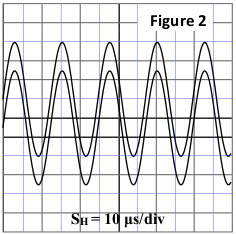
\includegraphics[width=0.32\textwidth]{./img/ex4_2.png}
  \end{center}
\end{wrapfigure}

\textbf{1.1- }Choisir la proposition juste, parmi les propositions
suivantes :

\textbf{a- }Les ondes ultrasonores sont des ondes
électromagnétiques.

\textbf{b- }Les ondes ultrasonores ne se propagent pas dans le vide.

\textbf{c- }Le phénomène de diffraction ne peut pas être obtenu par les ondes ultrasonores.

\textbf{d- }Les ondes ultrasonores se propagent dans l’air avec une vitesse égale à la célérité de la lumière

\textbf{1.2- }Déterminer la fréquence N de l’onde ultrasonore étudiée.

\textbf{1.3- }Vérifier que la vitesse de propagation de l’onde ultrasonore dans l’air est $V_a = 340 m/s$.

\textbf{2- Détermination de la vitesse de propagation d’une onde ultrasonore dans l’eau de mer\dotfill}

L’émetteur envoie l’onde ultrasonore précédente dans deux tubes, l’un contenant de l’air l’autre étant
rempli d’eau de mer (figure 3). Le récepteur $R_1$ capte l’onde qui se propage dans l’air et le récepteur capte l’onde qui se propage dans de mer.
  \begin{center}
	  \vspace{-0.3cm}
	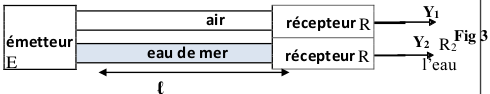
\includegraphics[width=0.6\textwidth]{./img/ex4_3.png}
	  \vspace{-0.4cm}
  \end{center}

\begin{wrapfigure}{r}{0.36\textwidth}
  \begin{center}
	  \vspace{-0.8cm}
	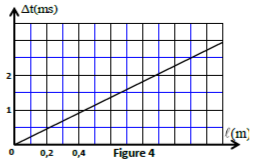
\includegraphics[width=0.36\textwidth]{./img/ex4_4.png}
  \end{center}
\end{wrapfigure}


Soient $\Delta{t}$ le retard temporel de réception de l’onde qui se
propage dans l’air par rapport à celle qui se propage dans l’eau
de mer et $l$ la distance entre l’émetteur et les deux récepteurs.

En mesurant le retard $\Delta{t}$ pour différentes distances entre
L’émetteur et les deux récepteurs (figure 3), on obtient la
courbe de la figure 4.

\textbf{2.1- }Exprimer $\Delta{t}$ en fonction de $l$, $V_a$ et $V_e$ vitesse de
propagation de l’onde dans l’eau de mer.

\textbf{2.2- }Déterminer la valeur de $V_e$.
\end{Box2}


\begin{Box2}{Exercice 5:la propagation des ondes mécaniques à la surface de l'eau }

	\begin{wrapfigure}[7]{r}{0.36\textwidth}
  \begin{center}
	  %\vspace{-0.8cm}
	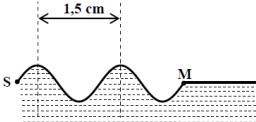
\includegraphics[width=0.36\textwidth]{./img/ex5.png}
  \end{center}
\end{wrapfigure}


\emph{Pour étudier la propagation des ondes mécaniques à la surface de l'eau, on utilise une cuve à ondes.
Le but de cette partie de l’exercice est de déterminer quelques
grandeurs caractéristiques d'une onde mécanique.}

A l'aide d'un vibreur d'une cuve à ondes, on crée en un point S
de la surface libre de l'eau une onde progressive sinusoïdale de
fréquence N = 20 Hz. Cette onde se propage à t = 0 à partir
du point S, sans amortissement et sans réflexion.

La figure ci-contre représente une coupe, dans un plan vertical, d'une partie de la surface de l'eau à
l'instant de date $t_1$.

\textbf{1- }L'onde qui se propage à la surface de l'eau est-elle transversale ou longitudinale ? Justifier.

\textbf{2-}Déterminer la longueur d'onde $\lambda$ de l'onde étudiée.

\textbf{3- } Déduire la célérité V de l'onde à la surface de l'eau.

\textbf{4- } Le point M, situé à la distance $d=SM$ du point S, est le front de l'onde à l'instant de date $t_1$. Exprimer le retard temporel $\tau$ du mouvement de M par rapport au mouvement de S, en fonction de la période T de l'onde. Calculer $\tau$.



\end{Box2}


\begin{Box2}{Exercice 6: le mouvement des vagues}

	\begin{wrapfigure}{r}{0.26\textwidth}
  \begin{center}
	  %\vspace{-0.8cm}
	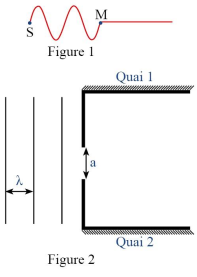
\includegraphics[width=0.26\textwidth]{./img/ex6.png}
  \end{center}
\end{wrapfigure}


\emph{Les vents créent aux larges des océans des vagues qui se propagent vers les côtes. Le but de cet exercice
est d’étudier le mouvement de ces vagues}

On considère que les ondes se propageant à la surface des eaux des mers sont progressives et
sinusoïdales de période T = 7 s.

\textbf{1- }L’onde étudiée est-elle longitudinale ou transversale ? Justifier.

\textbf{2- }Calculer V, la vitesse de propagation de ces ondes, sachant
que la distance séparant deux crêtes consécutives est d = 70 m.

\textbf{3- }La figure 1 modélise une coupe verticale de l’aspect de la
surface de l’eau à un instant t.

On néglige le phénomène de dispersion, et on considère S comme
source de l’onde et M son front loin de S de la distance SM.

\textbf{3.1- }A l’aide de la figure 1, écrire l’expression du retard
temporel $\tau$ du mouvement de M par rapport à S en
fonction de la longueur d’onde $\lambda$. Calculer la valeur de $\tau$.

\textbf{3.2- }Préciser, en justifiant, le sens du mouvement de M à
l’instant où l’onde l’atteint.

\textbf{4- }Les ondes arrivent à un portail de largueur a = 60 m situé entre
deux quais d’un port (Figure 2). Recopier le schéma de la figure 2, et représenter dessus les ondes après la traversée du portail, et donner le nom du phénomène observé.



\end{Box2}

\begin{Box2}{Exercice 7 : Propagation d’une onde ultrasonore dans l’air }

\textbf{1- Etude de la propagation d’une onde ultrasonore\dotfill}

Pour étudier la propagation des ondes ultrasonores dans l’eau, on utilise le montage suivant (figure1) E un émetteur et R un récepteur

\begin{center}
	  %\vspace{-0.8cm}
	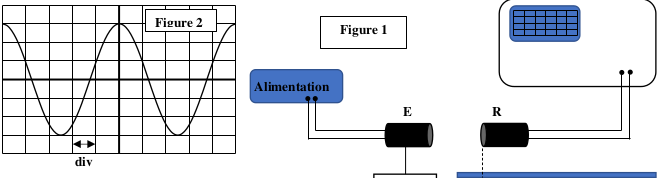
\includegraphics[width=0.76\textwidth]{./img/ex7.png}
  \end{center}

\textbf{1.1- }Définir une onde mécanique progressive.

\textbf{1.2- }L’onde ultrasonore est-elle une onde longitudinale ou transversale ? Justifier la réponse

\textbf{1.3- }La courbe de la figure 2 représente les variations de la tension aux bornes du récepteur R, la sensibilité horizontale est $S_h=2\mu{s}/div$

\textbf{1.3.1- }Déterminer graphiquement la valeur de la période T de l’onde reçus par le récepteur R
\textbf{1.3.2- }Déterminer la valeur $\lambda$ de la longueur d’onde sachant que la vitesse de propagation de l’onde sonore dans l’aire est : $V_{air}=340m/s$

\textbf{2- Détermination de la profondeur des eaux :\dotfill}

\emph{Un sondeur acoustique classique (Le sonar) est composé d’une sonde comportant un émetteur et un récepteur d’onde ultrasonore. la sonde envoie une onde ultrasonore verticalement en direction du
fond.}

\emph{Cette onde ultrasonore se déplace dans l’eau à une vitesse constante veau. Et quand elle
rencontre un obstacle, une partie de l’onde est réfléchie et renvoyée vers la source. La détermination du retard entre l’émission et la réception du signal permet de calculer la profondeur p.}

Pour déterminer la profondeur de l'eau dans un port, un navire envoi à l’aide d’un émetteur E, un signal ultrasonore périodique vers le fond de la mer. le signal réfléchit sur le fond est capté par un récepteur (Figure3) le schéma de la figure 4 représente le signal émis par E et le signal reçu par R
visualisé par un appareil convenable.

\textbf{2.1- }Déterminer $\Delta{t}$ La durée qui sépare l’instant de l’envoi du signal et l’instant de la réception de la partie réfléchie.

\textbf{2.2- }On considère que les ultrasons suivent une trajectoire verticale. Déduire la valeur de d la profondeur de l’eau dans l’endroit où se trouve le bateau, sachant la vitesse de propagation de l’onde ultrasonore dans l’eau est : $V_{eau} = 1,5 .10^3m/s$

  \begin{center}
	  %\vspace{-0.8cm}
	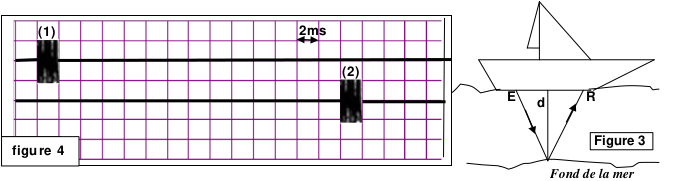
\includegraphics[width=0.86\textwidth]{./img/ex7_1.png}
  \end{center}

\end{Box2}

%\begin{wrapfigure}{r}{0.22\textwidth}
  %\begin{center}
	  %\vspace{-0.6cm}
	%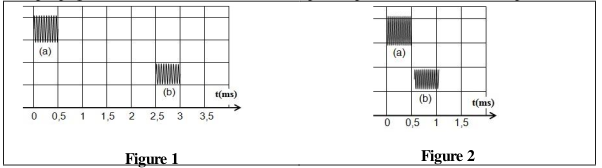
\includegraphics[width=0.22\textwidth]{./img/Ex2.png}
  %\end{center}
%\end{wrapfigure}
%\vspace{2cm}
%\begin{center}
   %\Large{ \em{Exercices Supplémentaires}}
%\end{center}


%\vspace{-0.7cm}
%%_________________________Exercice 5 : _________________________Exercice
%\begin{Box2}{Exercice 5 :Les ondes sonores }
%4
%\end{Box2}
%%_________________________Exercice 6 : _________________________Exercice
%\begin{Box2}{Exercice 6 : échographie}
%6
%\end{Box2}

\end{document}
